\xchapter{Referencial Teórico}{}

\acresetall 
O presente capítulo apresenta os conceitos fundamentais necessários para a compreensão do trabalho proposto: evolução de software; qualidade de software; teste de software; teste de regressão, e técnicas de seleção de teste de regressão.

\section{Evolução de Software}\label{sec:evolucaodesoftware}


O desenvolvimento de um software não termina com a entrega do sistema, mas, refere-se a um processo contínuo durante toda a sua vida útil. Após a entrega do sistema, para que ele se mantenha útil, faz-se necessário o processo de evolução do software. A \textbf{evolução} é a fase em que as mudanças significativas na arquitetura e nas funcionalidades do software podem ser feitas. 
No processo de evolução, ao decorrer da utilização do software, surgem novas solicitações de mudança, gerando assim novas \textit{releases} do sistema.

Uma das consequências da evolução de software é a constante necessidade de realizar sua manutenção. A Norma IEEE 1219 \cite{257623} define manutenção de software como a modificação de um produto de software após a entrega para corrigir falhas; melhorar o desempenho ou outros atributos; ou adaptar o produto a uma modificação. \citeonline{DBLP:series/springer/Mens08} classifica o processo de manutenção como: perfectiva, corretiva, adaptativa ou preventiva:

\begin{itemize}
   
    \item \textbf{Manutenção perfectiva}: É qualquer modificação de um produto de software após a entrega com o objetivo de melhorar o desempenho ou a capacidade de manutenção.
   
    \item \textbf{Manutenção corretiva}: Diz respeito às modificações reativas de um produto de software executadas após a entrega para corrigir falhas descobertas.
   
    \item \textbf{Manutenção adaptativa}: É a modificação de um produto de software executada após a entrega para manter um programa de computador utilizável em um ambiente modificado ou em mudança.
   
    \item \textbf{Manutenção preventiva}: Refere-se a modificações de software realizadas com o objetivo de prevenir problemas antes que eles ocorram.

\end{itemize}


\section{Qualidade de Software}\label{sec:qualidadedesoftware}


O termo qualidade é apresentado com diferentes conceitos na literatura. A ISO 9000 define qualidade como o grau
em que um conjunto de características inerentes preenchem os requisitos \cite{iso9000}. Para \citeonline{juran1970quality} e \citeonline {crosby1979quality}, o conceito de qualidade está relacionado à ``conformidade com requisitos'' e ``adequação para
uso'', respectivamente. Para \citeonline{HIRAMA2011}, qualidade é algo difícil de ser definido. Ainda mais difícil é garantir a qualidade de algum produto, visto que a percepção de qualidade passa pelas expectativas que cada pessoa tem sobre algum produto ou serviço. 

Tendo em vista a importância da qualidade no processo de desenvolvimento de um software, garantir a qualidade é uma tarefa relevante. Segundo \citeonline{HIRAMA2011}, Garantia de Qualidade, é o processo geral de definição de como a qualidade de software pode ser atingida e como a organização de desenvolvimento sabe que o software tem o nível de qualidade necessário. A garantia de qualidade estabelece processos, procedimentos e padrões que conduzem a um software de qualidade. 

De acordo com \citeonline{HIRAMA2011}, a qualidade de um software está intimamente relacionada à quantidade de defeitos descobertos. Quanto mais defeitos são descobertos, maior é a qualidade do software. 


\section{Teste de Software}\label{sec:testesdesoftware}
Apresentamos alguns conceitos necessários para compreensão da importância da atividade de teste.

\subsection{Validação, Verificação e Teste}

Em geral, dividem-se as atividades de Validação, Verificação e Teste em estáticas e dinâmicas. As estáticas são as que não requerem a execução ou mesmo a existência de um programa ou modelo executável para serem conduzidas. As dinâmicas são as que se baseiam na execução de um programa ou de um modelo \cite{DELAMARO2007}.

\ac{VV} permite que se determine sistematicamente se os requisitos de um sistema estão sendo corretamente tratados e implementados. Por sua vez, a atividade de testes tem por objetivo descobrir defeitos no software, considerando aspectos estruturais e lógicos. \ac{VV} contribuem diretamente para o atendimento dos prazos e custos do projeto. Portanto, conhecer os conceitos de \ac{VV} é importante para obter produtos de maior qualidade e produtividade e melhorar os processos continuamente. As atividades de verificar, validar e testar auxiliam na Garantia da Qualidade do software \cite{HIRAMA2011}.


É importante compreender a distinção entre alguns conceitos relacionados, conforme apresentado no padrão de testes de software da IEEE \cite{159342}:

\begin{enumerate}
    \item \textbf{Erro \textit{(error, mistake)}:} Uma ação humana que produz um resultado incorreto.
    
    \begin{itemize}
        \item Os desenvolvedores cometem erros (enganos) quando interpretam mal as necessidades dos clientes.
        \item Os usuários cometem erros (enganos) quando operam um sistema em desacordo com as intenções dos desenvolvedores.
    \end{itemize}
    
    \item \textbf{Defeito \textit{(bug, fault, defect)}:} Implementado dentro de um artefato.
    
    \begin{itemize}
        \item Requisitos inconsistentes com as necessidades dos clientes.
        \item Requisitos funcionais do sistema em desacordo com os requisitos de
negócio.
    \end{itemize}
    
     \item \textbf{Falha \textit{(failure)}:} A incapacidade de um sistema ou componente em executar
as funções requeridas dentro de um nível de desempenho requerido.

    \begin{itemize}
        \item Manifestação de um defeito no sistema ou software (ex: a ``tela azul'' no Sistema Operacional Windows).
    \end{itemize}
    
\end{enumerate}

\subsection{Atividade de Teste de Software}

A atividade de teste tem por objetivo descobrir defeitos no software, considerando aspectos estruturais e lógicos. O teste de software pode ser usado para mostrar a presença de defeitos, mas nunca a sua ausência \cite{HIRAMA2011}.

Testes devem acontecer desde o momento da concepção do software perpassando todo o processo de desenvolvimento. Um procedimento de teste completo é composto por algumas etapas, conforme apresentado na Figura \ref{figure:PTESTE}. O teste procura descobrir defeitos quando o comportamento do software não está correto ou não está em conformidade com o que foi especificado.

\begin{figure}[!htb]
\centering
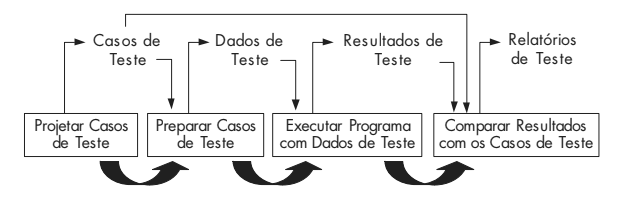
\includegraphics[width=.8\textwidth]{images/PTESTE.png}
\caption{Procedimento de Teste \cite{HIRAMA2011}}
\label{figure:PTESTE}
\end{figure}

Um dos resultados do procedimento de teste é gerar os casos de teste para que posteriormente possam ser executados.  Um bom caso de teste é aquele que tem uma grande probabilidade de revelar um defeito ainda não descoberto \cite{HIRAMA2011}.

O documento básico para a atividade de teste é o Plano de Testes, no qual se define: objetivos para cada tipo (ou fase de teste); estratégias de teste; cronograma e responsabilidades; procedimentos e padrões a serem usados na execução e na elaboração do relatório de testes; critérios para a conclusão do teste, bem como o sucesso de cada teste \cite{HIRAMA2011}.

A execução dos testes pode ser feita de forma manual, quando a partir de um roteiro a ser seguido é feita por um profissional de forma manual, ou pode ser feita de forma automatizada, com a utilização de ferramentas que executam os testes e reportam os resultados. Para \citeonline{Ammann:2008:IST:1355340}, o teste de software é caro e exige mão de obra intensiva, e requer até 50\% dos custos de desenvolvimento de software e ainda mais para aplicativos críticos de segurança. Faz-se necessário automatizar o máximo possível dos testes de software, reduzindo significativamente o custo, minimizando o erro humano e facilitando o teste de regressão.


\subsection{Técnicas de Teste de Software}


Segundo \citeonline{DELAMARO2007}, as duas técnicas mais amplamente aceitas na academia e na indústria são as técnicas de testes \textit{funcionais} e as \textit{estruturais}, comumente conhecidas como teste Caixa Preta e teste Caixa Branca, respectivamente. Elas são discutidas a seguir:



\begin{itemize}
    \item \textbf{Técnica Funcional}: Técnica utilizada para projetar casos de teste na qual o programa ou sistema é considerado uma caixa preta. Para testá-lo, fornece-se entradas e avalia-se as saídas geradas para verificar se estão em conformidade com os objetivos especificados. No teste funcional os detalhes de implementação não são considerados e o software é avaliado segundo a visão do usuário \cite{DELAMARO2007}.
    
    \item \textbf{Técnica Estrutural}: A técnica estrutural estabelece os requisitos de teste com base em uma dada implementação, requerendo a execução de partes ou de componentes elementares do programa. Testa-se os caminhos lógicos do software, utilizando casos de teste para provar conjuntos específicos, estruturas condicionais, definições e uso de variáveis. Os testes gerados por essa técnica são chamados também de teste de caixa branca \cite{DELAMARO2007}.
    
\end{itemize}

Segundo \citeonline{HIRAMA2011}, os testes de Caixa Branca e os testes de Caixa Preta precisam atender algumas características, que são elas:\\

\textbf{Características dos testes Caixa Branca:}

\begin{itemize}
    \item O projeto de casos de teste usa a estrutura de controle procedimental do software (fluxo de controle do software) para derivar casos de teste;
    \item Deve garantir que todos os caminhos independentes dentro de um módulo tenham sido exercitados pelo menos uma vez;
    \item Deve exercitar todas as decisões lógicas para valores falsos ou verdadeiros;
    \item Deve executar todos os laços em suas fronteiras e dentro de limites operacionais;
    \item Deve exercitar as estruturas de dados internas para garantir a sua validade.
\end{itemize}



\textbf{Características dos testes Caixa Preta:}

\begin{itemize}
    \item Concentram-se nos requisitos funcionais do software;
    \item São uma abordagem complementar aos testes estruturais.
\end{itemize}


\subsection{Tipos de Teste}


A atividade de testes é dividida em fases com objetivos distintos \cite{DELAMARO2007}. Segundo \citeonline{HIRAMA2011}, os tipos de teste mais comuns realizados para cobrir os testes estruturais e funcionais são: teste de unidade (estrutural); teste de integração (funcional); teste de validação (funcional); e teste de sistema (funcional).

\begin{itemize}

\item {\textbf{Teste de unidade}}: tem como foco as menores unidades de um programa, podendo ser funções, procedimentos, métodos ou classes. O objetivo é testar os componentes isoladamente verificando o funcionamento conjunto dos algoritmos e as estruturas de dados. Espera-se então que sejam identificados erros relacionados a algoritmos incorretos ou mal implementados, estruturas de dados incorretas, ou simples erros de programação.  A referência usada para os testes é a Especificação de Módulos, um documento detalhado de cada módulo de software. O teste de unidade pode ser aplicado à medida que ocorre a implementação das unidades e pelo próprio desenvolvedor. 

\item {\textbf{Teste de integração}}: deve ser realizado após serem testadas as unidades individuais, e a ênfase é dada na construção da estrutura do sistema. O objetivo é testar um conjunto de módulos verificando o seu funcionamento com foco nas suas interfaces entre os módulos. Quando as diversas partes do software são colocadas para trabalhar juntas, verifica-se se a interação entre elas funciona de maneira adequada e não ocasiona erros. Faz-se necessário um grande conhecimento das estruturas internas e das interações existentes entre as partes do sistema. A referência usada para os testes é a Especificação de Projeto, um documento detalhado da organização e interdependência entre os módulos de software. O teste de integração tende a ser executado pela própria equipe de desenvolvimento. 

\item {\textbf{Teste de validação}}: tem como objetivo testar o software como um todo verificando se todas as exigências funcionais, comportamentais e de desempenho foram atendidas. A referência usada para os testes é a Especificação de Requisitos de Software, um documento que contém os requisitos funcionais e não funcionais do software. O teste é realizado pela equipe de desenvolvimento de software.

\item {\textbf{Teste de sistema}}: tem como objetivo medir o sistema em diferentes cenários verificando se todos os elementos do sistema (hardware, software, banco de dados e pessoas) foram adequadamente integrados e realizam as funções requeridas. A referência usada para os testes é a Especificação de Sistema, um documento que contém a descrição funcional do sistema, dos subsistemas e do seu desempenho no ambiente operacional. O teste é realizado por uma equipe independente ou um usuário do sistema.

\end{itemize}

Segundo \citeonline{HIRAMA2011}, existem ainda outros testes que podem ser aplicados a sistemas de software. São eles: teste de recuperação, teste de proteção, teste de estresse, teste de desempenho, dentre outros, que visam validar requisitos não-funcionais do software, i.e., aqueles ligados aos atributos de qualidade esperados. Alguns desses são descritos a seguir:

\begin{itemize}
    
    \item \textbf{Teste de recuperação}: teste que força o sistema a apresentar falhas de diversas maneiras e verifica se a recuperação (reiniciação do sistema e recuperação de dados) é adequadamente executada.
    
    \item \textbf{Teste de proteção}: teste que tenta verificar se todos os mecanismos de proteção embutidos em um sistema funcionam contra acessos indevidos.
    
    \item \textbf{Teste de estresse}: teste para confrontar o software com situações anormais (alta exigência de recursos, alto número de interrupções, alta taxa de entrada de dados, alta busca de dados em disco).
    
    \item \textbf{Teste de desempenho}: teste de software no contexto de um sistema integrado (tempos envolvidos, ciclos de processador, interrupções).

\end{itemize}

Outros tipos de teste de software relevantes são os testes \textbf{alfa} e \textbf{beta}, que estão relacionados ao teste de aceitação. Em virtude das dificuldades encontradas pelos desenvolvedores para preverem como o cliente usará o programa, ou, como ele irá interpretar os manuais de usuários, alguns testes são realizados para compreender como será a aceitação do cliente em relação ao software desenvolvido. 


\section{Teste de Regressão}\label{sec:testesregressao}

\subsection{Definição}

 A \citeonline{159342} define teste de regressão como repetição seletiva de um sistema ou componente para verificar se as modificações não causaram efeitos não-intencionais e se o sistema ou componentes ainda estão em conformidade com o requisito especificado. Segundo \citeonline{Ammann:2008:IST:1355340}, o teste de regressão é o processo de testar novamente o software que foi modificado. 
 
 À medida que os desenvolvedores mantêm um sistema de software, eles periodicamente fazem teste de regressão, na esperança de encontrar erros causados por suas alterações e fornecer confiança de que suas modificações estão corretas. Para suportar esse processo, os desenvolvedores geralmente criam um conjunto inicial de testes, que são reutilizáveis. A estratégia de teste de regressão mais simples é a reexecução de todos os casos de teste. Essa abordagem, porém, torna-se provavelmente inviável por exigir uma quantidade muito grande de tempo para a sua execução completa \cite{Graves:2001:ESR:367008.367020}. Para \citeonline{Ammann:2008:IST:1355340} o teste de regressão constitui a grande maioria dos esforços de teste no desenvolvimento de software comercial, e é uma parte essencial de qualquer processo de desenvolvimento de software viável.
 
 Segundo \citeonline{LEUNG1989}, os testes de regressão podem ser corretivos ou progressivos. A Tabela \ref{table:TRCP} apresenta algumas diferenças fundamentais entre ambos.

 
\begin{table}[th]
    \footnotesize
    \centering
    \caption{Teste de Regressão Corretivo \& Progressivo \cite{LEUNG1989}}
    \label{table:TRCP}
    \def \arraystretch{1.3}
    \begin{tabular}{m{6.5cm}m{6.5cm}}
        \toprule
        \textbf{Teste de Regressão Corretivo} & \textbf{Teste de Regressão Progressivo} \\
        \midrule
        \textit{A especificação não é alterada} & A especificação é alterada\\
        \textit{Envolve pequenas modificações no código (por exemplo, adicionar e excluir instruções)} & Envolve modificação importante (por exemplo, adicionar e excluir módulos)\\ 
        \textit{Geralmente feito durante o desenvolvimento e a manutenção corretiva} & Geralmente feito durante a manutenção adaptativa e aperfeiçoada\\
        \textit{Muitos casos de teste podem ser reutilizados} & Menos casos de teste podem ser reutilizados\\
        \textit{Chamado em intervalos irregulares} & Chamado em intervalos regulares\\
        \bottomrule
    \end{tabular}
\end{table}

Para \citeonline{Ammann:2008:IST:1355340}, os testes de regressão devem ser automatizados. De fato, pode-se dizer que o teste de regressão não automatizado é equivalente a nenhum teste de regressão.


\subsection{Distinção entre as classes de técnicas}
 
Para \citeonline{Ammann:2008:IST:1355340}, uma técnica é \textbf{precisa} na medida em que omite testes de regressão que não são reveladores de modificação. Uma técnica é \textbf{eficiente} na medida em que determinar o subconjunto apropriado do conjunto de testes de regressão. Por sua vez, uma técnica é \textbf{geral} no grau que se aplica a uma ampla variedade de situações práticas.

Segundo \citeonline{Yoo:2012:RTM:2284811.2284813}, as técnicas de teste de regressão são classificadas como: Técnicas de Seleção; Técnicas de Minimização; e Técnicas de Priorização, seguida das seguintes definições:
 
 
\begin{itemize}
 
 \item \textbf{Definição 1 (Problema de Minimização do Conjunto de Testes)}:
 
 As técnicas de minimização do conjunto de testes visam identificar casos de teste redundantes e removê-los do conjunto de testes para reduzir o tamanho do conjunto de testes.
  
\textbf{Dado}: Um conjunto de testes $T$, um conjunto de requisitos de teste ${r1, ..., rn}$, que deve ser satisfeito para fornecer o teste ``adequado'' desejado do programa e subconjuntos de ${T, T1, ..., T_n}$, um relacionado a cada um dos $r_is$ de tal forma que qualquer um dos casos de teste $t_j$ pertencentes ao $T_$ pode ser usado para atingir o requisito $r_i$.

\textbf{Problema}: Encontre um conjunto representativo, $T'$, de casos de teste de $T$ que satisfaça todos os $r_is$.



\item \textbf{Definição 2 (Problema de Seleção de Casos de Teste)}:

A seleção do caso de teste, do original em inglês \ac{RTS}, é essencialmente semelhante ao problema de minimização do conjunto de testes: ambos os problemas tratam da escolha de um subconjunto de casos de teste do conjunto de testes. A principal diferença entre essas duas abordagens na literatura é se o foco está nas mudanças no sistema sob teste, do original em inglês \ac{SUT}. A minimização do conjunto de testes geralmente é baseada em métricas como a cobertura medida de uma única versão do programa em teste. Em contraste, no \ac{RTS}, os casos de teste são selecionados porque sua execução é relevante para as mudanças entre a versão anterior e a atual do \ac{SUT}.

\textbf{Dado}: O programa $P$, a versão modificada de $P$, $P'$ e um conjunto de testes $T$.
\textbf{Problema}: Encontre um subconjunto de  $T$ , $T'$, com o qual testar $P'$.



\item \textbf{Definição 3 (Problema de Priorização de Casos de Teste)}:

A priorização de caso de teste procura encontrar o pedido ideal de casos de teste para teste, para que o testador obtenha o máximo benefício, mesmo se o teste for prematuramente interrompido em algum ponto arbitrário. 

\textbf{Dado}: Um conjunto de testes $T$, o conjunto de permutações de $T$, $PT$ e uma função de $PT$ para números reais, $f: PT \longrightarrow R$.

\textbf{Problema}: Para encontrar $T' \in PT \longrightarrow (\forall T")(T" \in PT)(T" \ne T')[f(T') \geq  f(T")]$.


\end{itemize}


\subsection{Classificação dos casos de teste}


\citeonline{Yoo:2012:RTM:2284811.2284813} categorizam os casos de teste em cinco classes. As três primeiras classes consistem em casos de teste que já existem em $T$.

\begin{itemize}
  \item \textbf{Reutilizável}: Os casos de teste reutilizáveis executam apenas as partes do programa que permanecem inalteradas entre duas versões, ou seja, as partes do programa que são comuns a $P$ e $P'$. Não é necessário executar esses casos de teste para testar $P'$; no entanto, eles são chamados de reutilizáveis porque ainda podem ser retidos e reutilizados para o teste de regressão das futuras versões do $P$.
  \item \textbf{Retestável}: Casos de teste retestáveis executam as partes de P que foram alteradas em $P'$. Assim, os casos de teste retestáveis devem ser reexecutados para testar $P'$.
  \item \textbf{Obsoleto}: Os casos de teste podem se tornar obsoletos porque (1) sua relação de entrada / saída não é mais correta devido a mudanças nas especificações, (2) eles não testam mais o que foram projetados para testar devido a modificações no programa ou (3) casos de teste ``estruturais'' que não mais contribuem para a cobertura estrutural do programa.

As duas classes restantes consistem em casos de teste que ainda precisam ser gerados para o teste de regressão de $P'$.

\item \textbf{Novo-estrutural}: Novos casos de teste estrutural testam as construções modificadas do programa, fornecendo cobertura estrutural das partes modificadas em $P'$.


\item \textbf{Nova especificação}: Casos de teste de nova especificação testam as especificações do programa modificado, testando o novo código gerado a partir das partes modificadas das especificações de $P'$.
\end{itemize}

\section{Técnicas de seleção de teste de regressão}\label{sec:rts}


Em virtude da necessidade de técnicas \textbf{eficientes}, que determinam o subconjunto apropriado de casos de teste a serem reexecutados, e de técnicas \textbf{precisas} que omitem casos de teste que não são reveladores de modificação \cite{Ammann:2008:IST:1355340}, ao longo de décadas diversos estudos foram realizados para prover essas técnicas \cite{WHITE1991}, \cite{Graves:2001:ESR:367008.367020}, \cite{630875}, \cite{536955}, \cite{ENGSTROM201014},\cite{ENGSTROM201014}, \cite{KAZMI2017}, \cite{ROMANO201862}.

As técnicas podem ser categorizadas, para que sejam avaliadas e comparadas, em quatro categorias: inclusividade, precisão, eficiência e generalidade. A \textbf{inclusividade} mede o quanto uma técnica escolhe testes que farão com que o programa modificado produza uma saída diferente do programa original expondo falhas causadas por modificações. A \textbf{precisão} mede a capacidade de uma técnica evitar a escolha de testes que não farão com que o programa modificado produza resultados diferentes do programa original. A \textbf{eficiência} mede o custo computacional e, portanto, a praticidade de uma técnica. A \textbf{generalidade} mede a capacidade de uma técnica lidar com construções de linguagem realistas e diversificadas, modificações de código arbitrariamente complexas e aplicativos de teste realistas \cite{536955}.

As técnicas de seleção reduzem o custo do teste de um programa modificado, pois, reutilizam testes existentes e identificam partes do programa modificado ou sua especificação que deve ser testada. Estas técnicas diferem da técnica de reexecução de todos os casos de teste da versão original. \citeonline{WHITE1991} uma técnica de seleção é mais econômica que a técnica de reexecução de todos os casos de teste, se o custo de selecionar um subconjunto reduzido de testes a executar for menor que o custo de executar os testes que a técnica de seleção omitir.

Os procedimentos fundamentais executados por uma técnica de seleção de teste de regressão são: \cite{536955}

\begin{enumerate}
    \item Selecionar $T'$ $\subseteq$ $T$, um conjunto de casos de teste para executar em $P'$.
    \item Testar $P'$ com $T'$, para estabelecer a correção de $P'$ em relação a $T'$.
    \item Se necessário, criar $T''$, um novo conjunto de casos de teste funcional ou estrutural para testar $P'$.
    \item Testar $P'$ com $T''$, para estabelecer a correção de $P'$ em relação a $T''$.
    \item Crie $T'''$, um novo conjunto de casos de teste e histórico de testes para $P'$, de $T$, $T'$, e $T''$.
\end{enumerate}

Executando essas etapas, uma técnica de seleção de teste de regressão aborda quatro problemas. A etapa 1 refere-se ao problema de selecionar um subconjunto de testes $T'$ de $T$ com o qual possa testar $P'$. A etapa 3 refere-se ao problema de cobertura, ou seja, identificar a necessidade de criação de testes adicionais. As etapas 2 e 4 tratam o problema de executar testes com eficiência, verificando se os resultados estão corretos. A etapa 5 refere-se ao problema de manutenção do conjunto de testes, atualizando e armazenando as informações de teste.

As técnicas de seleção de teste de regressão tem como foco o problema 1, ou seja, selecionar um subconjunto de teste de $T$ representado por $T'$ com o qual testar $P'$, garantindo assim que as mudanças realizadas não modificaram o funcionamento do software. Essas técnicas localizam testes em $T$ que expõem falhas em $P'$.

Algumas premissas fundamentais em relação a técnicas de seleção de teste de regressão: \cite{536955}
\begin{itemize}
    \item Um teste $t$ detecta uma falha em $P'$ se ele faz com que $P'$ falhe. Neste caso pode-se dizer que $t$ é um revelador de falhas de $P'$.
    \item Um programa $P$ falha em $t$ se, quando $P$ for testado com $t$, $P$ produzir uma saída incorreta de acordo com $S$.
    \item Uma técnica de seleção de teste de regressão pode selecionar um subconjunto do conjunto de testes em $T$ que revelam falhas para $P'$. Nessas condições pode-se dizer que essa técnica não omite testes em $T$ que possam revelar falhas em $P'$.
    \item Um teste $t$ é revelador de modificações para $P$ e $P'$ se, e somente se, faz com que as saídas de $P$ e $P'$ sejam diferentes.
    \item O teste $t$ é considerado obsoleto para o programa $P'$ se e somente se $t$ especificar uma entrada para $P'$ que, de acordo com $S'$, é inválida para $P'$ ou $t$ especificar uma relação de entrada-saída inválida para $P'$.
\end{itemize}


\section{Testes de apps para Android}\label{testesAndroid}

Segundo \citeonline{glauber2019dominando}, o Android não é apenas um sistema operacional, mas um conjunto completo de software para dispositivos móveis que inclui: um sistema operacional, um \textit{middleware} e aplicações-chave. O Android é open-source e seu código fonte está disponível para download \footnote{\url{https://source.android.com/}}. Assim como o código-fonte, a documentação para desenvolvimento e teste também está disponível para consulta\footnote{\url{https://developer.android.com/}} . 

Desenvolver e testar apps para Android apresentam alguns desafios específicos, tais como: concorrência, segurança, performance, eficiência energética, compatibilidade, detecção de defeitos \cite{8453877}. Assim, testar um app para Android é uma tarefa que tende a exigir um esforço da equipe. 

Com o objetivo de reduzir o esforço de teste no processo de desenvolvimento de \ac{APPS} para Android, tanto a literatura, quanto o mercado, propõem ferramentas para automatizar o processo de testes em \ac{APPS} Android. As ferramentas podem ser gratuitas ou proprietárias, e estão focadas em diferentes tipos de testes no processo de desenvolvimento dos \ac{APPS}. O Apêndice \ref{table:androidtools} apresenta vinte e cinco ferramentas utilizadas para testes de apps para Android.

\section{Síntese do Capítulo}\label{sec:sintesecapitulo}

O presente capítulo apresentou os conceitos fundamentais para compreensão do estudo proposto. Na Seção \ref{sec:evolucaodesoftware} abordamos sobre o processo de evolução de software. Na Seção \ref{sec:qualidadedesoftware} definimos o conceito de qualidade e sua importância no processo de desenvolvimento de software. A Seção \ref{sec:testesdesoftware} apresenta diversos conceitos sobre teste de software. Na Seção \ref{sec:testesregressao} tratamos sobre uma técnica distinta de testes, denominada teste de regressão. Na Seção \ref{sec:rts} tratamos sobre as técnicas de seleção de teste de regressão. E na Seção \ref{testesAndroid} abordarmos sobre a atividade de testes em \ac{APPS} para Android. No próximo capítulo apresentaremos o \textit{Survey} realizado com profissionais e pesquisadores que atuam em projetos de \ac{APPS} para Android.